\documentclass{article}
\usepackage[utf8]{inputenc}
\usepackage{graphicx}
\graphicspath{ {./images/} }

\title{AM1 - Zestaw 9}
\author{wojciech185sz }
\date{April 2020}

\begin{document}

\maketitle

\section{Zadanie 1, (f)}

$$r(x) = \frac{sin^{2}x}{x^3}$$
Dziedziną tejże funkcji są wszystkie liczby rzeczywiste poza zerem. \newline
$\displaystyle\lim_{x \to -\infty} \frac{sin^{2}x}{x^3} = 0 = \displaystyle\lim_{x \to +\infty}\frac{sin^{2}x}{x^3}$ \newline
$\displaystyle\lim_{x \to 0^-} \frac{sin^{2}x}{x^3} = -\infty $ \newline
$\displaystyle\lim_{x \to 0^+} \frac{sin^{2}x}{x^3} = +\infty $ \newline \newline

Z powyższego wynika, że prosta x = 0 jest asymptotą pionową obustronną funkcji, a prosta y = 0 jest jej asymptotą poziomą w $-\infty$ oraz $+\infty$ (odp.)

\section{Zadanie 2, (e)}
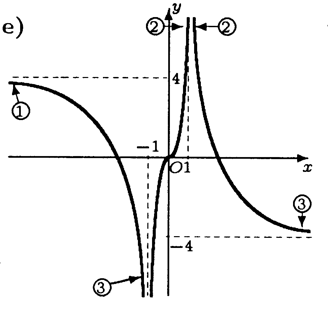
\includegraphics{wykres.png}

\section{Zadanie 4, (a)}

$$e^{\frac{x+y}{2}} \leq \frac{e^{x}+e^{y}}{2}$$

Rozważmy punkty: $A = (x, e^x)$, $B = (y, e^y)$. Połączmy je prostą, której środek oznaczymy przez $C = (\frac{x+y}{2}, \frac{e^{x}+e^{y}}{2}$. Z wypukłości środek (C) jest nad wartością funkcji $e^{\frac{x+y}{2}}$. Co nakazano dowieść.

\end{document}